\documentclass[aspectratio=169, 11pt]{beamer}

% --- Packages & Setup ---
\usepackage[utf8]{inputenc}
\usepackage[T1]{fontenc}
\usepackage{helvet}
\renewcommand{\familydefault}{\sfdefault}
\usepackage{xcolor}
\usepackage{booktabs}
\usepackage{graphicx}
\usepackage{tikz}
\usetikzlibrary{calc, arrows.meta}

% small picture inside an architecture box (variant B)
\newcommand{\archpic}[1]{\includegraphics[width=1.55cm,height=0.9cm,keepaspectratio]{#1}}

\graphicspath{{../}{./}{figures/}}

% A figure is shown when the file exists; otherwise a labelled box marks where it goes.
\newcommand{\figorbox}[3]{%
  \IfFileExists{figures/#1}{\includegraphics[width=#2]{figures/#1}}{%
    \fbox{\begin{minipage}[c][3.2cm]{#2}\centering\scriptsize\textbf{[#3]}\end{minipage}}}}

% --- Branding Colors ---
\definecolor{amritaMaroon}{HTML}{A4123F}

% --- Theme Setup ---
\usetheme{Madrid}
\usecolortheme[named=amritaMaroon]{structure}
\setbeamertemplate{navigation symbols}{}
\setbeamertemplate{footline}[frame number]

% Shared styles for the TikZ diagrams (moved up from slide 5 so every slide can use them).
\tikzset{
    archbox/.style={draw=amritaMaroon, thick, rounded corners=3pt, fill=amritaMaroon!8, align=center,
        font=\scriptsize, text width=1.65cm, minimum height=1.25cm, inner sep=4pt},
    archbottom/.style={draw=amritaMaroon, thick, rounded corners=3pt, fill=amritaMaroon!8, align=center,
        font=\scriptsize, text width=2.4cm, minimum height=1.3cm, inner sep=5pt},
    archarr/.style={-{Latex[length=2mm]}, thick, amritaMaroon},
    archsection/.style={font=\small\bfseries, text=amritaMaroon},
    archlab/.style={font=\tiny, text=black!85, fill=white, inner sep=2pt, align=center}
}

\begin{document}

% ===================== PAGE 1: TITLE =====================
\begin{frame}
    \begin{tikzpicture}[remember picture,overlay]
        \node[fill=amritaMaroon, text=white, font=\bfseries\footnotesize, anchor=north east, rounded corners=2pt, inner sep=5pt]
        at ($(current page.north east) + (-0.2cm,-0.2cm)$)
        {Type 2: Application Project};
    \end{tikzpicture}

    \centering
    \includegraphics[width=2.4cm]{logo.png}
    \vspace{0.05cm}

    {\large \textbf{\textcolor{amritaMaroon}{Autonomous First-Response Crime Scene Exploration\\Using a Lightweight Onboard Intelligence System}}} \\
    \vspace{0.05cm}
    {\footnotesize \textbf{23CSE498 -- Project Phase II (External Review)} \quad | \quad \textbf{Team Number: G040}} \\
    \vspace{0.1cm}

    \begin{table}
        \centering
        \scriptsize
        \renewcommand{\arraystretch}{1.0}
        \begin{tabular}{|c|c|l|}
            \hline
            \textbf{S.No} & \textbf{Register Number} & \textbf{Student Name} \\
            \hline
            1 & CB.SC.U4CSE23062 & Karthik Raju \\
            \hline
            2 & CB.SC.U4CSE23063 & Maheswar Raju \\
            \hline
            3 & CB.SC.U4CSE23112 & Vijay Krishna Burra \\
            \hline
            4 & CB.SC.U4CSE23310 & Dhinesh Chandra Boddupally \\
            \hline
            5 & CB.SC.U4CSE23421 & Kuchipudi Yokshith Sai Ram \\
            \hline
        \end{tabular}
    \end{table}
    \vspace{0.05cm}

    {\footnotesize Guide: \textbf{Mr. Rajeshwar Yadav}, Assistant Professor, Department of CSE} \\
    \vspace{0.05cm}
    {\scriptsize \today}
\end{frame}

% ===================== PAGE 2: GUIDE APPROVAL =====================
\begin{frame}{Guide Review \& Submission Approval}
    \framesubtitle{Confirmation of Project Review and Approval from Guide}
    \centering
    \fbox{\begin{minipage}[c][5.4cm]{0.94\textwidth}
        \centering
        \textbf{[Insert Screenshot of Guide Approval Email Here]} \\[0.3cm]
        {\footnotesize [Mandatory: Attach a clear, readable screenshot of the email received from your project guide approving this presentation and final review submission]}
    \end{minipage}}
\end{frame}

\section{Requirements \& Solution Design}

% ===================== PAGE 3: PROBLEM DEFINITION =====================
\begin{frame}{1. Problem Definition }
    \framesubtitle{Target Problem \& User Needs}
    \begin{block}{Problem Statement \& Target Stakeholders}
        \small
        \begin{itemize}
            \item \textbf{Real-World Problem:} before entering a crime scene, hostage site or collapsed building, responders have no map of the inside, cannot safely see what is behind walls and doors, and do not know what kind of incident it is; sending people in first puts both the responders and the evidence at risk.
            \item \textbf{Target Users \& Use Context:} police first-response and forensic teams, search-and-rescue and disaster-response units; a four-legged robot goes in first, maps the place and reports what it sees before any person enters.
        \end{itemize}
    \end{block}
\end{frame}

% ===================== PAGE 4: REQUIREMENT ANALYSIS =====================
\begin{frame}{2. Requirement Analysis}
    \framesubtitle{Functional / Non-Functional Requirements}
    \begin{block}{Functional Requirements}
        \small
        \begin{itemize}
            \item \textbf{FR-1:} explores an unknown place without an operator and returns to its start point with a map of the building.
            \item \textbf{FR-2:} tracks its own position and builds a floor map using one depth camera, a gyro and leg movements.
            \item \textbf{FR-3:} from camera video, detects whether a crime is happening, the kind of emergency, and which of 13 crimes it is.
        \end{itemize}
    \end{block}

    \begin{block}{Non-Functional Requirements \& Constraints}
        \small
        \begin{itemize}
            \item \textbf{NFR-1:} real time: 20 Hz control loop, median 29 ms per step on a CPU, no GPU.
            \item \textbf{NFR-2:} safety: zero collisions, recovery from every stall, same code in every environment.
        \end{itemize}
    \end{block}
\end{frame}

% ===================== PAGE 5: END-TO-END ARCHITECTURE =====================
\begin{frame}{3. End-to-End Application Architecture}
\framesubtitle{System Architecture \& Sensor-to-Action Workflow}
\centering
\resizebox{\textwidth}{!}{%
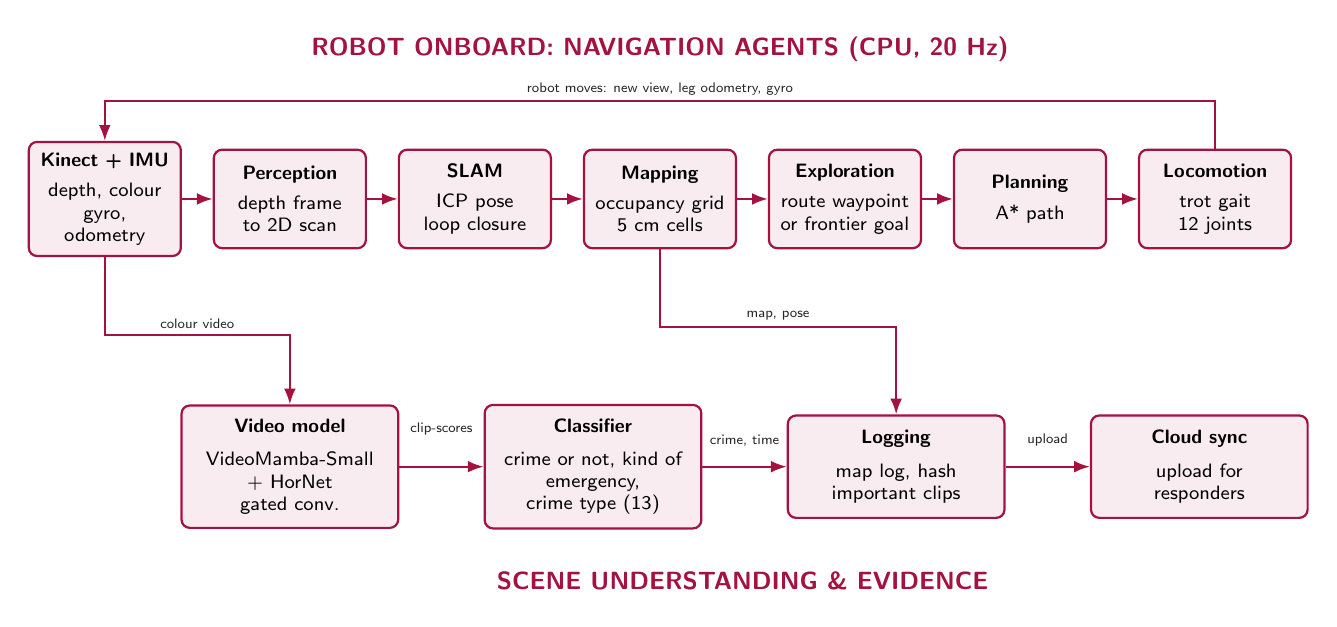
\begin{tikzpicture}

% section headings
\node[archsection] at (8.15,3.35) {ROBOT ONBOARD: NAVIGATION AGENTS (CPU, 20 Hz)};
\node[archsection] at (9.2,-3.40) {SCENE UNDERSTANDING \& EVIDENCE};

% top row: sensing to legs
\node[archbox] (kin)  at (1.1,1.45)   {\textbf{Kinect + IMU}\\[3pt]depth, colour\\gyro, odometry};
\node[archbox] (per)  at (3.45,1.45)  {\textbf{Perception}\\[3pt]depth frame\\to 2D scan};
\node[archbox] (slam) at (5.8,1.45)   {\textbf{SLAM}\\[3pt]ICP pose\\loop closure};
\node[archbox] (map)  at (8.15,1.45)  {\textbf{Mapping}\\[3pt]occupancy grid\\5 cm cells};
\node[archbox] (fro)  at (10.5,1.45)  {\textbf{Exploration}\\[3pt]route waypoint\\or frontier goal};
\node[archbox] (plan) at (12.85,1.45) {\textbf{Planning}\\[3pt]A* path};
\node[archbox] (loco) at (15.2,1.45)  {\textbf{Locomotion}\\[3pt]trot gait\\12 joints};

\draw[archarr] (kin.east) -- (per.west);
\draw[archarr] (per.east) -- (slam.west);
\draw[archarr] (slam.east) -- (map.west);
\draw[archarr] (map.east) -- (fro.west);
\draw[archarr] (fro.east) -- (plan.west);
\draw[archarr] (plan.east) -- (loco.west);

% closed loop: moving changes what the sensors see
\draw[archarr] (loco.north) -- ++(0,0.6) -| node[pos=0.25, above, archlab] {robot moves: new view, leg odometry, gyro} (kin.north);

% bottom row: scene understanding and evidence
\node[archbottom] (vid)   at (3.45,-1.95) {\textbf{Video model}\\[4pt]VideoMamba-Small\\+ HorNet gated conv.};
\node[archbottom] (cls)   at (7.3,-1.95)  {\textbf{Classifier}\\[4pt]crime or not, kind of\\emergency, crime type (13)};
\node[archbottom] (log)   at (11.15,-1.95) {\textbf{Logging}\\[4pt]map log, hash\\important clips};
\node[archbottom] (cloud) at (15.0,-1.95) {\textbf{Cloud sync}\\[4pt]upload for\\responders};

\draw[archarr] (vid.east) -- node[above=9pt, archlab] {clip-scores} (cls.west);
\draw[archarr] (cls.east) -- node[above=5pt, archlab] {crime, time} (log.west);
\draw[archarr] (log.east) -- node[above=5pt, archlab] {upload} (cloud.west);

% colour video from the Kinect; map and pose to the log
\draw[archarr] (kin.south) -- ++(0,-0.99) -| node[pos=0.25, above, archlab] {colour video} (vid.north);
\draw[archarr] (map.south) -- ++(0,-0.99) -| node[pos=0.25, above, archlab] {map, pose} (log.north);
\end{tikzpicture}}

\vspace{0.07cm}
{\scriptsize Agents never call each other: they exchange the latest messages on one publish-subscribe bus.}
\end{frame}

% ===================== PAGE 8: COMPONENTS & USER WORKFLOW =====================
\begin{frame}{4. Architectural Components \& Interface Design}
    \framesubtitle{Component Breakdown \& User Workflow}
    \begin{block}{Core Application Components}
        \small
        \begin{itemize}
            \item \textbf{SLAM:} lets the robot find where it is while building a map of an unknown place. Our robot does this with one depth camera, a gyro and its leg movements.
            \item \textbf{Exploration:} goes to the edges of unexplored areas, takes the shortest safe path and passes through narrow gaps.
            \item \textbf{Scene understanding:} VideoMamba-Small with a HorNet gated convolution; tells crime or not, the kind of emergency and the crime type.
        \end{itemize}
    \end{block}

    \begin{block}{User Interaction \& Workflow Design}
        \small
        \begin{itemize}
            \item \textbf{Primary User Journey:} the responder places the robot at the entrance, optionally marks a route and starts; the robot explores and returns with the map.
            \item \textbf{Interface Design:} a live map with the robot's path while it explores; at the end, the finished map, the crime type with the moment it is most visible, and a mission report.
        \end{itemize}
    \end{block}
\end{frame}

% ===================== PAGE 9: DATA & PLATFORM =====================
\begin{frame}{5. Architectural Components \& Interface Design}
    \framesubtitle{Data Management, Interfaces \& Technology Specifications}
    \begin{block}{Data Management \& External Interfaces}
        \small
        \begin{itemize}
            \item \textbf{Data Storage:} each mission saves the map, the robot's path, an event timeline, a knowledge graph of rooms and doorways, and video clips tagged with the crime type and time; the sensor data is recorded so a mission can be replayed and checked later.
            \item \textbf{External Interfaces:} Kinect depth and colour camera, gyro, leg odometry and the 12 leg joints.
        \end{itemize}
    \end{block}

    \begin{block}{Platform \& Deployment Specifications}
        \small
        \begin{itemize}
            \item \textbf{Development Stack:} Python 3.12, NumPy, OpenCV for navigation; Python 3.10, PyTorch 2.1 and mamba\_ssm for scene understanding; CoppeliaSim for testing.
            \item \textbf{Deployment Target:} navigation was run and tested on a laptop CPU; Scene understanding runs on a GPU (Tesla V100).
        \end{itemize}
    \end{block}
\end{frame}

% ===================== PAGE 10: IMPLEMENTATION OVERVIEW =====================
\begin{frame}{6. Implementation Details: Overview}
    \framesubtitle{End-to-End Application Module \& Integration Status}
    \begin{table}
        \centering
        \scriptsize
        \renewcommand{\arraystretch}{1.2}
        \begin{tabular}{p{3.4cm} p{7.4cm} c}
            \toprule
            \textbf{Application Module} & \textbf{Implemented Features \& Integration Scope} & \textbf{Status} \\
            \midrule
            Operator interface & Start the mission, mark an optional search route, watch the live map; read the mission report and report the crime.& 100\% (Functional) \\
            SLAM \& exploration & Seven agents on one shared message bus. The robot explores and returns to its start point. & 100\% (Integrated) \\
            Scene understanding & Trained network: crime or not, kind of emergency, crime type, and the moment it is most visible & 100\% (Functional) \\
            Data storage & Each mission saves the map, path, event timeline and sensor recording; a mission can be replayed and checked later & 100\% (Integrated) \\
            Sensors \& motors & Kinect depth and colour camera, gyro, leg odometry, 12 leg joints, collision check & 100\% (Functional, sim) \\
            \bottomrule
        \end{tabular}
    \end{table}

    \begin{block}{Prototype Environment \& Repository}
        \footnotesize
        \begin{itemize}
            \item \textbf{Execution Platform:} navigation tested in the CoppeliaSim simulator on Windows 11 (AMD Ryzen 7, CPU only); scene understanding on a Tesla V100 GPU.
            \item \textbf{Source Repository:} github.com/yokshith09/Autonomous-Quadruped-SLAM-Navigation-Perception (tag final-multi-env-v2); github.com/vijaykrishnaaa/VideoMamba-HorNet-Crime-Recognition
        \end{itemize}
    \end{block}
\end{frame}

% ===================== PAGE 7: SCENE-UNDERSTANDING NETWORK =====================
\begin{frame}{7. End-to-End Application Architecture (Scene Understanding)}
    \framesubtitle{VideoMamba-Small with a HorNet Gated Convolution}
    \centering
    \figorbox{fig_recognition_model.png}{0.97\textwidth}{Recognition network: figures/fig\_recognition\_model.png}
    \vspace{0.1cm}
    \begin{block}{Architecture Summary}
        \footnotesize An 8-frame clip becomes spatio-temporal patches, passes 24 bidirectional Mamba layers (last 8 with a HorNet gated convolution) and is classified into 13 crimes or Background.
    \end{block}
\end{frame}

% ===================== PAGE 12: SCENE UNDERSTANDING IMPLEMENTATION =====================
\begin{frame}{8. Functional Module Implementation Details}
    \framesubtitle{Scene Understanding: From Video to Answer}
    \begin{block}{Scene Understanding}
        \small
        \begin{itemize}
            \item \textbf{Implemented Workflow:} a video is cut into 60 short clips at four scales; the four strongest clips for each crime decide the answer.
            \item \textbf{Inputs \& Outputs:} colour video in; crime or not, kind of emergency, top-3 crimes and the strongest moment out.
            \item \textbf{Validation \& Controls:} the model and the crime cut-off are chosen on separate validation videos; test videos are used once; if the top two crimes are very close, the answer says \emph{not sure}.
        \end{itemize}
    \end{block}

    \vspace{0.3cm}
    \centering
    \resizebox{0.92\textwidth}{!}{%
    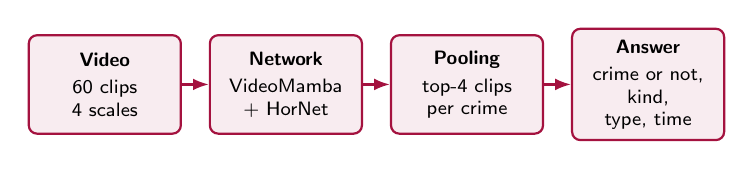
\begin{tikzpicture}
        \node[archbox] (v) at (0,0)   {\textbf{Video}\\[2pt]60 clips\\4 scales};
        \node[archbox] (n) at (2.3,0) {\textbf{Network}\\[2pt]VideoMamba\\+ HorNet};
        \node[archbox] (p) at (4.6,0) {\textbf{Pooling}\\[2pt]top-4 clips\\per crime};
        \node[archbox] (a) at (6.9,0) {\textbf{Answer}\\[2pt]crime or not,\\kind, type, time};
        \draw[archarr] (v.east) -- (n.west);
        \draw[archarr] (n.east) -- (p.west);
        \draw[archarr] (p.east) -- (a.west);
    \end{tikzpicture}}
\end{frame}

% ===================== PAGE 16: DEMO, SCENE UNDERSTANDING =====================
\begin{frame}{9. Working Prototype Demonstration: Scene Understanding}
    \framesubtitle{One Command, One Video, Three-Level Answer}
    \begin{columns}[c]
        \column{0.24\textwidth}
        \centering
        \figorbox{fig_demo_input.png}{\linewidth}{Input video frames: figures/fig\_demo\_input.png}\\[2pt]
        {\scriptsize \textbf{Input:} 14 s, 442 frames}



        \column{0.66\textwidth}
        \centering
        \figorbox{fig_demo_output.png}{\linewidth}{Scene-understanding output: figures/fig\_demo\_output.png}\\[2pt]
        {\scriptsize \textbf{Output:} three-level answer printed by one command}
    \end{columns}
    \vspace{0.2cm}

    \begin{block}{Live Demonstration Scenario}
        \footnotesize
        \begin{itemize}
            \item \textbf{Crime or not:} crime score 0.90, above the 0.68 cut-off, so it is flagged as a crime.
            \item \textbf{Crime type:} Arrest and Burglary tie at 24\%, so the answer is shown as unsure; true label is Burglary.
            \item \textbf{Kind of emergency and strongest moment:} Violence or Property, most visible at 6.4 to 6.9 s.
        \end{itemize}
    \end{block}
\end{frame}

% ===================== PAGE 6: ROBOT CORE ARCHITECTURE =====================
\begin{frame}{10. End-to-End Application Architecture (Navigation)}
\framesubtitle{Robot Core: Seven Agents on One Message Bus}
\centering
\resizebox{\textwidth}{!}{%
\begin{tikzpicture}[
    agent/.style={draw=amritaMaroon, thick, rounded corners=3pt, fill=amritaMaroon!8, align=center,
        font=\small, text width=2.7cm, minimum height=3.6cm, inner sep=4pt},
    busbox/.style={draw=amritaMaroon, thick, rounded corners=3pt, fill=amritaMaroon!20, align=center,
        font=\small, minimum height=0.9cm, inner sep=3pt},
    biarr/.style={{Latex[length=2.5mm]}-{Latex[length=2.5mm]}, thick, amritaMaroon},
    oneway/.style={-{Latex[length=2.5mm]}, thick, amritaMaroon}
]

% ---------- six navigation agents: name, picture, then text below the picture ----------
\node[agent] (per)  at (0,2.6)    {\textbf{Perception}\\[3pt]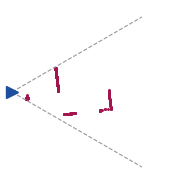
\includegraphics[width=2.6cm,height=1.9cm,keepaspectratio]{icon_scan.png}\\[2pt]{\scriptsize 10 Hz\\depth frame to 2D scan}};
\node[agent] (slam) at (3.3,2.6)  {\textbf{SLAM}\\[3pt]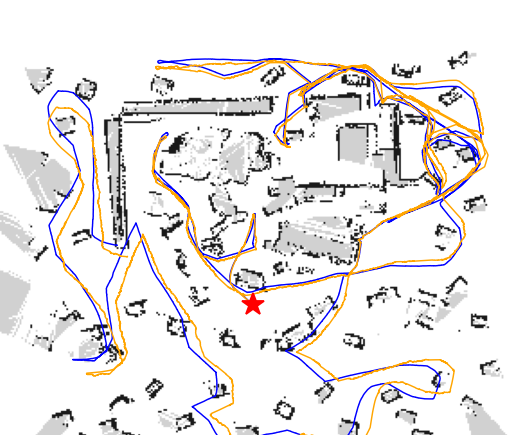
\includegraphics[width=2.6cm,height=1.9cm,keepaspectratio]{img_map2.png}\\[2pt]{\scriptsize 10 Hz\\ICP pose, loop closure}};
\node[agent] (map)  at (6.6,2.6)  {\textbf{Mapping}\\[3pt]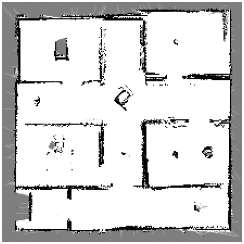
\includegraphics[width=2.6cm,height=1.9cm,keepaspectratio]{icon_grid.png}\\[2pt]{\scriptsize 10 Hz\\occupancy grid, rooms}};
\node[agent] (fro)  at (9.9,2.6)  {\textbf{Frontier}\\[3pt]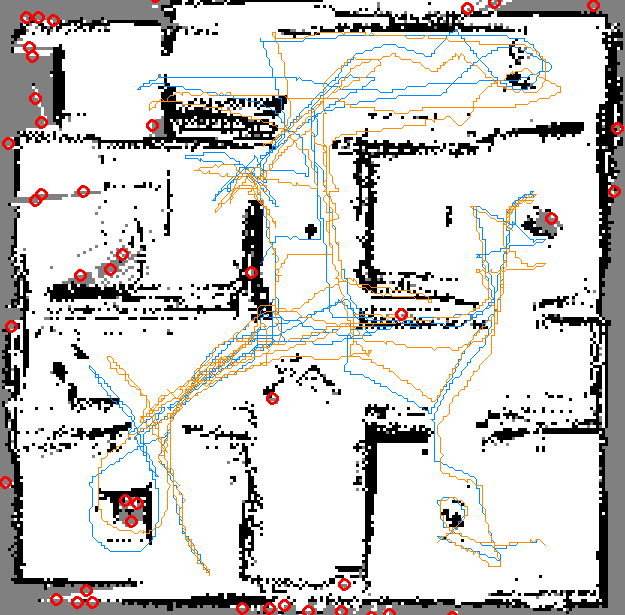
\includegraphics[width=2.6cm,height=1.9cm,keepaspectratio]{img_map.png}\\[2pt]{\scriptsize 1 Hz\\route or frontier goal}};
\node[agent] (plan) at (13.2,2.6) {\textbf{Planning}\\[3pt]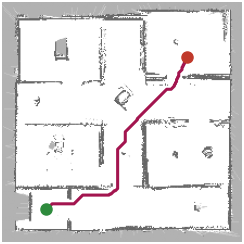
\includegraphics[width=2.6cm,height=1.9cm,keepaspectratio]{icon_path.png}\\[2pt]{\scriptsize 5 Hz\\A* path}};
\node[agent] (loco) at (16.5,2.6) {\textbf{Locomotion}\\[3pt]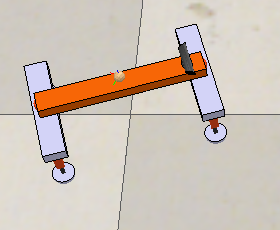
\includegraphics[width=2.6cm,height=1.9cm,keepaspectratio]{img_robot.png}\\[2pt]{\scriptsize 20 Hz\\trot gait, watchdog}};

% ---------- message bus ----------
\node[busbox, minimum width=19.6cm] (bus) at (8.25,-0.55)
    {\textbf{MESSAGE BUS (publish / subscribe)}\quad{\scriptsize one 20 Hz scheduler runs every agent at its own rate; agents never call each other}};

\foreach \a in {per, slam, map, fro, plan, loco}
    \draw[biarr] (\a.south) -- (\a.south |- bus.north);

% ---------- camera, supervisor, leg joints ----------
\node[agent, minimum height=3.0cm] (kin) at (0,-3.4)
    {\textbf{Kinect camera}\\[3pt]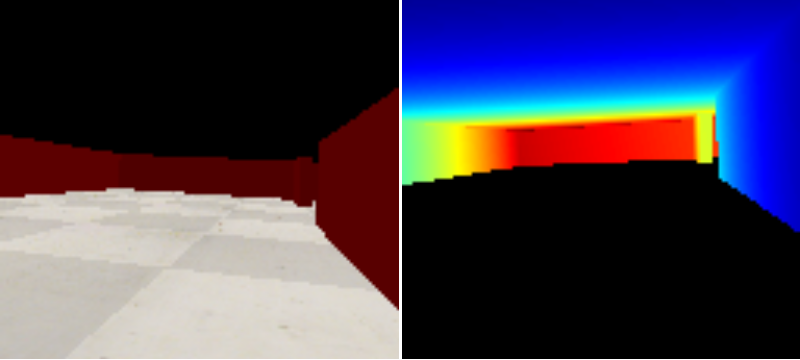
\includegraphics[width=2.6cm,height=1.6cm,keepaspectratio]{img_rgbd.png}\\[2pt]{\scriptsize depth + colour frames}};
\node[agent, text width=4.4cm, minimum height=3.0cm] (sup) at (8.25,-3.4)
    {\textbf{Supervisor agent}\\[4pt]{\scriptsize 2 Hz\\[2pt]mission state, knowledge graph of rooms, event timeline}};
\node[agent, minimum height=3.0cm] (leg) at (16.5,-3.4)
    {\textbf{12 leg joints}\\[3pt]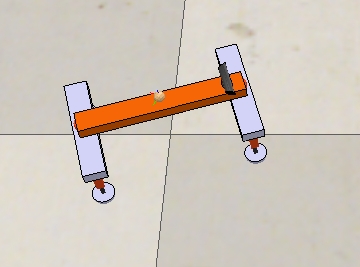
\includegraphics[width=2.6cm,height=1.6cm,keepaspectratio]{robot_sim.png}\\[2pt]{\scriptsize joint angles from the gait}};

\draw[oneway] (kin.north) -- (kin.north |- bus.south);
\draw[biarr]  (sup.north) -- (sup.north |- bus.south);
\draw[oneway] (leg.north |- bus.south) -- (leg.north);
\end{tikzpicture}}
\end{frame}

% ===================== PAGE 11: NAVIGATION AGENTS =====================
\begin{frame}{11. Functional Module Implementation Details}
    \framesubtitle{Navigation: What Each Agent Does}
    \small
    \begin{itemize}
        \setlength{\itemsep}{2.8pt}
        \item \textbf{Perception:} turns the camera's depth frame into a 2D obstacle scan, after removing the floor and the robot's own body.
        \item \textbf{SLAM:} uses the scan, leg movement and gyro to find the robot's position, trusting a scan match only if it agrees with the legs.
        \item \textbf{Mapping:} uses the scan and position to build a 5 cm floor map with rooms and doors, marking a wall only after repeated readings.
        \item \textbf{Frontier:} uses the map to pick the next route point or unexplored area, skips places it cannot reach, and returns the robot to the start at the end.
        \item \textbf{Planning:} uses the map and goal to find the shortest path, passing only through cells a safe distance from walls.
        \item \textbf{Locomotion:} follows the path with a trot gait to drive the 12 leg joints, turning away if stuck and stopping before floor edges.
        \item \textbf{Supervisor:} uses position, map and events to track the mission and write the report.
    \end{itemize}

    \vspace{0.2cm}
    {\footnotesize Agents never call each other: each shares its result on one message bus and reads the others' latest results.}
\end{frame}

\section{Functional Testing \& Demonstration}

% ===================== PAGE 14: BENCHMARKS =====================
\begin{frame}{12. Functional Testing \& Verification Results (Benchmarks)}
    \framesubtitle{Same Data, Same Scoring: Where the System Stands}
    \begin{columns}[T]
        \column{0.50\textwidth}
        \begin{block}{Localisation on our recordings (ATE)}
            \scriptsize
            \begin{tabular}{lcc}
                \toprule
                \textbf{Method} & \textbf{Scene 1 / 2} & \textbf{Average} \\
                \midrule
                Odometry only & 291.4 / 15.7 cm & 153.6 cm \\
                BreezySLAM (best of 11) & 189.7 / 109.5 cm & 149.6 cm \\
                Cartographer (best of 8) & 341.5 / 85.2 cm & 213.4 cm \\
                \textbf{Ours} & \textbf{11.7 / 12.3 cm} & \textbf{12.0 cm} \\
                \bottomrule
            \end{tabular}

            {\tiny Same recordings for every method: best run per scene (scene 2: 12-min run). Full final runs: 14.8 / 28.8 cm, average 21.8 cm.}
        \end{block}
        \begin{block}{Exploration vs nearest-frontier (same scenes)}
            \scriptsize
            Floor covered 90.0 vs 78.7\%; stuck 3 vs 12.5 per run; only ours passed through the building.
        \end{block}

        \column{0.46\textwidth}
        \begin{block}{Public TUM RGB-D Pioneer (ATE)}
            \scriptsize
            \begin{tabular}{lc}
                \toprule
                \textbf{System} & \textbf{Average} \\
                \midrule
                ORB-SLAM3 (published) & 172.0 cm \\
                OpenVSLAM (published) & 39.2 cm \\
                RTABMap (published) & 28.7 cm \\
                Wheel odometry only & 28.7 cm \\
                \textbf{Ours} & \textbf{25.9 cm} \\
                \bottomrule
            \end{tabular}
        \end{block}
        \begin{block}{UCF-Crime crime type (top-1)}
            \scriptsize
            Ours 43.10\% $\pm$ 1.47 (3 runs); Wu et al. CVPR 2024: 41.43\%; Anomize CVPR 2025: 47.14\% (both use CLIP).
        \end{block}
    \end{columns}
\end{frame}

% ===================== PAGE 13: FUNCTIONAL TESTING =====================
\begin{frame}{13. Functional Testing \& Verification Results}
    \framesubtitle{End-to-End Feature Verification \& Test Case Summary}
    \begin{table}
        \centering
        \scriptsize
        \renewcommand{\arraystretch}{1.15}
        \begin{tabular}{p{3.3cm} p{3.4cm} p{4.6cm} c}
            \toprule
            \textbf{Test Case / Feature} & \textbf{Test Input / Action} & \textbf{Verified Outcome} & \textbf{Status} \\
            \midrule
            TC-01: Exploration, building & Unknown 10 $\times$ 10 m building, 30 min & 94.2\% of floor, 0 collisions, ATE 14.8 cm & Pass \\
            TC-02: Route through a building & Rescue field, 70-waypoint route, 40 min & Through the building, 0 collisions, 5 stalls recovered & Pass \\
            TC-03: SLAM replay & Stored recordings replayed & Reproduces live error exactly & Pass \\
            TC-04: Boundary cases & Blocked waypoint, stall, floor edge & Skipped, recovered, stopped 0.44 m before edge & Pass \\
            TC-05: Crime or not & 290 UCF-Crime test videos & AUC 90.43\% & Measured \\
            TC-06: Crime type & 140 crime test videos & 43.10\% $\pm$ 1.47 & Measured \\
            TC-07: Kind of emergency & 140 crime test videos & 62.62\% (3 groups) & Measured \\
            \bottomrule
        \end{tabular}
    \end{table}

    \begin{block}{Application Verification Summary}
        \scriptsize
        \begin{itemize}
            \item \textbf{Functional Verification:} two environments, same code: 21.8 cm mean position error, 90.0\% floor covered, map F1 78.0\%, no collisions; 91 automated tests pass.
            \item \textbf{Responsiveness \& Operational Metrics:} 29 ms median control step on a CPU; scene understanding answers a 10 to 14 s video in 9 to 14 s on the GPU.
        \end{itemize}
    \end{block}
\end{frame}

% ===================== PAGE 15: DEMO, NAVIGATION =====================
\begin{frame}{14. Working Prototype Demonstration: Navigation}
    \framesubtitle{End-to-End Application Walkthrough \& Visual Evidence}
    \begin{columns}[c]
        \column{0.34\textwidth}
        \centering
        \href{https://drive.google.com/drive/folders/1RFVeb2BIp0LSHniS7wZZZ_BLYbO-NkT-?usp=sharing}{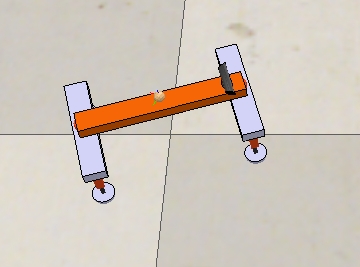
\includegraphics[width=\linewidth]{robot_sim.png}}\\[4pt]
        {\small \href{https://drive.google.com/drive/folders/1RFVeb2BIp0LSHniS7wZZZ_BLYbO-NkT-?usp=sharing}{\textcolor{amritaMaroon}{\textbf{$\blacktriangleright$ Click to play the run video}}}}

        \column{0.64\textwidth}
        \centering
        \includegraphics[width=\linewidth,height=4.4cm,keepaspectratio]{fig_scene2.png}\\[3pt]
        {\scriptsize Rescue field, 40 min: layout (left) and the robot's map (right); true path blue, estimated orange}
    \end{columns}

    \vspace{0.15cm}
    \begin{block}{Demonstration Scenario}
        \small The robot starts in the unknown rescue field, follows the operator's route through the damaged building, maps the field and returns to its start point.
    \end{block}
\end{frame}

\section{Technical Knowledge}

% ===================== PAGE 17: TECHNICAL JUSTIFICATION =====================
\begin{frame}{15. Technical Justification \& Architectural Decisions}
    \framesubtitle{Platform Rationale, Engineering Trade-offs \& Operational Considerations}
    \begin{columns}[T]
        \column{0.49\textwidth}
        \begin{block}{1. Platform \& Technology}
            \footnotesize
            \begin{itemize}
                \item One depth camera instead of lidar: cheaper, lighter, and it also gives colour video.
                \item Simulator gives the true position, so results are scored honestly.
                \item VideoMamba handles long clips faster than attention-based models.
            \end{itemize}
        \end{block}

        \begin{block}{2. Design Trade-offs}
            \footnotesize
            \begin{itemize}
                \item 2D scan keeps SLAM fast, but the 60\textdegree{} view sees little on open floor.
                \item Agents share one message bus: fast, and each can be replaced alone.
            \end{itemize}
        \end{block}

        \column{0.49\textwidth}
        \begin{block}{3. Safety \& Security}
            \footnotesize
            \begin{itemize}
                \item 0 collisions; keeps 0.5 m from unknown space; stops at floor edges; recovers when stuck.
                \item True position used only for scoring, never for driving.
                \item An unclear crime answer is shown as \emph{not sure}.
            \end{itemize}
        \end{block}

        \begin{block}{4. Limits \& Next Steps}
            \footnotesize
            \begin{itemize}
                \item Tested in simulation; error grows on long open floor; about 1 in 5 normal videos is flagged.
                \item Next: wider camera view, more rare-crime videos, real-robot tests.
            \end{itemize}
        \end{block}
    \end{columns}    \end{frame}

% =========================================================================
% REFERENCES & THANK YOU
% =========================================================================
\section{References}
\nocite{*}
\begin{frame}[allowframebreaks]{References}
    \bibliographystyle{ieeetr}
    \bibliography{ref}
\end{frame}

\begin{frame}
    \centering
    {\Huge \textbf{\textcolor{amritaMaroon}{Thank You}}} \\[0.4cm]
    {\large \textbf{Questions \& Viva Voce}}
\end{frame}

\end{document}
